% !TEX root = main.tex

% TODO:
% REMARK:

\section{Physical Objects Reconstruction and Selection}
\label{sec:PhysObj}

	\subsection{Vertex}
	\label{ssec:PhysObj_vertex}

		% https://iopscience.iop.org/article/10.1088/1742-6596/110/9/092009/pdf

	\subsection{Pileup Issue}
	\label{ssec:PhysObj_pu}{}

		% https://cms.cern/news/reconstructing-multitude-particle-tracks-within-cms
		Because of the high luminosity of pp collision in CMS, there are more than one pp collision occuring in every time when the the bunches cross one another. The multiple collision in one crossing event is called $\textbf{pile-up(pileup)}$. In the present, the LHC is operating at an instantaneous luminosity of $0.7\times10^{34} cm^{-2}s^{-1}$, and the proton bunches cross inside CMS every 50 ns, so there are more proton in one bunch and showing high pileup. Also, the high granularity and efficiency of CMS Tracker make them distinguish the many tracks in an event. The pileup image is shown below(Fig.\ref{PhysObj:fig:pileup_img}). There are more information in the reference \cite{Pileup_page}.

		% https://cms.cern/news/reconstructing-multitude-particle-tracks-within-cms
		\begin{figure}[H]
		\centering{}
	    	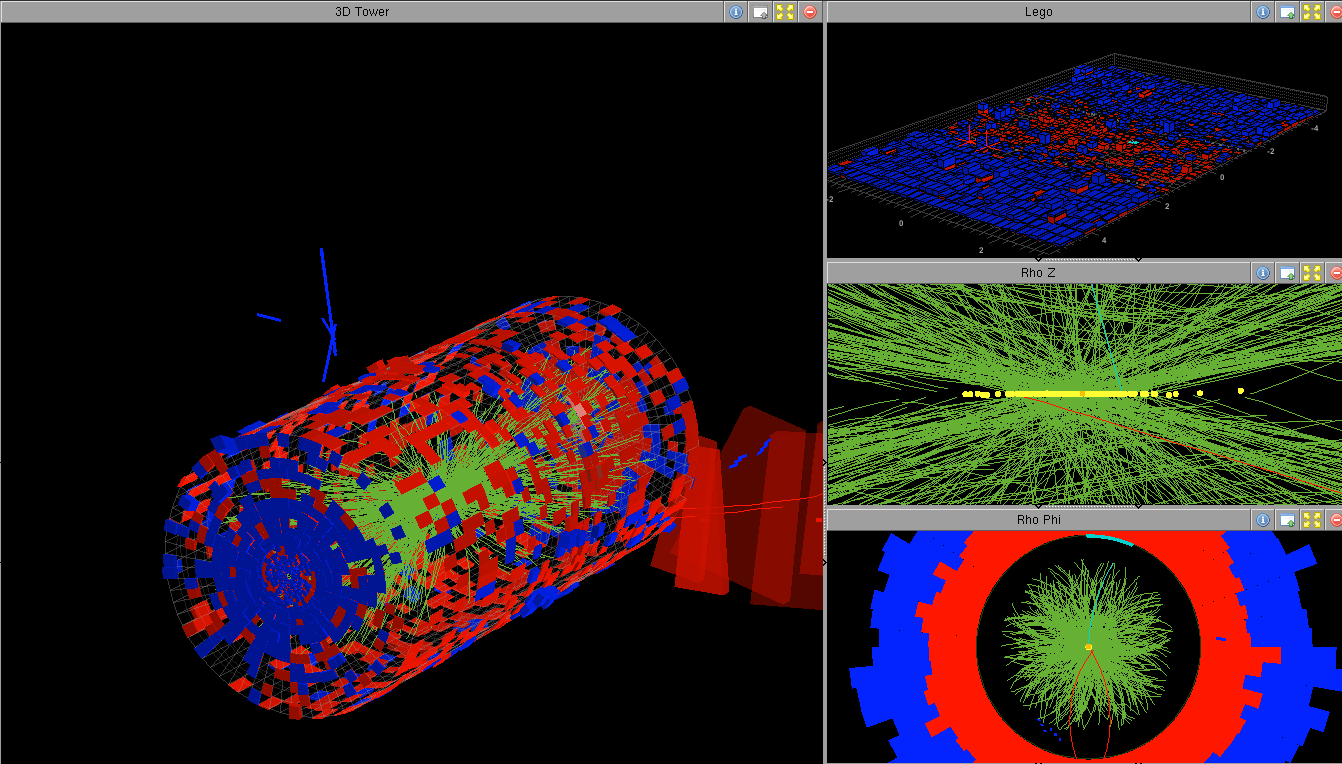
\includegraphics[width=0.85\textwidth]{Figures/PhysObj/pileup_image.png}\\
		\caption{78 reconstructed vertices in one crossing from high pileup run (3D, lego, on Pho-z plane, on Rho-Phi plane) \cite{Pileup_page}}
		\label{PhysObj:fig:pileup_img}
		\end{figure}
		\FloatBarrier



	\subsection{Lepton}
	\label{ssec:PhysObj_lep}

		The selected lepton in the analysis is required to obey the criteria of one passed $\emph{selected lepton}$ and zero $\emph{veto lepton}$ passed. The veto criteria means that there would be no lepton passing the veto criteria except the selected one. In other words, the veto criteria can filter the physical objects which are lepton-like but not really like after reconstructed from particle level to detector level. The selected criteria corresponds to tight lepton's criteria, and veto criteria follows loose lepton's criteria:

		\subsubsection{Muon}
		\label{sssec:Muon}
			

		\subsubsection{Electron}
		\label{sssec:Electron}

	\subsection{Jet}
	\label{ssec:PhysObj_jet}

		% Jet reco : Atkin_2015_J._Phys.__Conf._Ser._645_012008
		% anti-k algo : M. Cacciari, G. P. Salam, and G. Soyez, “The anti-k(t) jet clustering algorithm”, JHEP 04, 063 (2008)

		Jet is a type of physical object in high energy collider/detector physics. There are cluster of stable particles after collision, then fragmentating and hadronizing to be a jet. In the process, the strong interaction quarks and gluons cause the showering of these particles. And there is also some algorithm to reconstruct the showering to be an object -- jet, by some calormeter's and tracker's information.
		The used algorithm is anti-k algorithm to reconstruct all jets. The algorithm summarization is shown follow. First, there is a list of particles which are candidates of jets' member, they are called protojet. Secondly, for any i-th protojet, we find the minimum $d_{ij}$ and minimum $d_{iB}$ in the list. The $d_{ij}$ and $d_{iB}$ are defined below:

		\begin{equation}
		\begin{split}
		d_{ij} = min(P_{Ti}^{2p}, P_{Tj}^{2p}) \frac{\Delta_{ij}^2}{R^2}\\
		, \Delta_{ij} = \sqrt{ (\eta_i - \eta_j)^2 + (\phi_i - \phi_j)^2 }\\
		d_{iB} = P_{Ti}^{2p}
		\end{split}
		\label{eq:jet_reco_algo}
		\end{equation}
		\FloatBarrier

		In the definition, $P_{T}$, $\eta$ and $\phi$ individually means the transverse momentum, rapidity and azimuth of protojet. Also, the $\Delta_{ij}$ means the distance between i-th protojet and j-th protojet under $\eta$-$\phi$ space. Besides the radius parameter R, the p is the important parameter which decide the power of energy scale. The following step is to compare the minimum $d_{ij}$ and minimum $d_{iB}$, if the min-$d_{ij}$ is smaller than min-$d_{iB}$, then remove i-th and j-th protjets out of the list, and combine the i-th and j-th protojets into a new protojet and add in the original protojet list; if the min-$d_{ij}$ is larger than min-$d_{iB}$, then the i-th protojet is considered as a jet and remove it from the list of portojets. And then, choose the new i-th protojet and do the previous comparison and assignment again and again. The algorithm stops as long as the list of protojets is empty. The illustration example of algorithm is shown below(Fig.\ref{PhysObj:fig:jet_algo}). Furthermore, in CMS we commonly apply R by 0.4 as the AK4 jet, which is also used in the analysis. If the parameter $p=1$, it is called inclusive $k_{t}$ algorithm; and if $p=0$, Cambridge/Aachen algorithm; and if $p=-1$, anti-$k_{t}$ jet-clustering algorithm. For CMS, because of the high pileup property, it used to use $p=-1$ case -- anti-$k_{t}$ algorithm to construct jets. The behavior of different jet-reconstruction algorithm under $\eta$-$\phi$ space are shown in Fig.\ref{PhysObj:fig:3type_jetreco}. The informations are from \cite{Atkin_2015} and \cite{Cacciari_2008}.

		\begin{figure}[H]
		\centering{}
	    	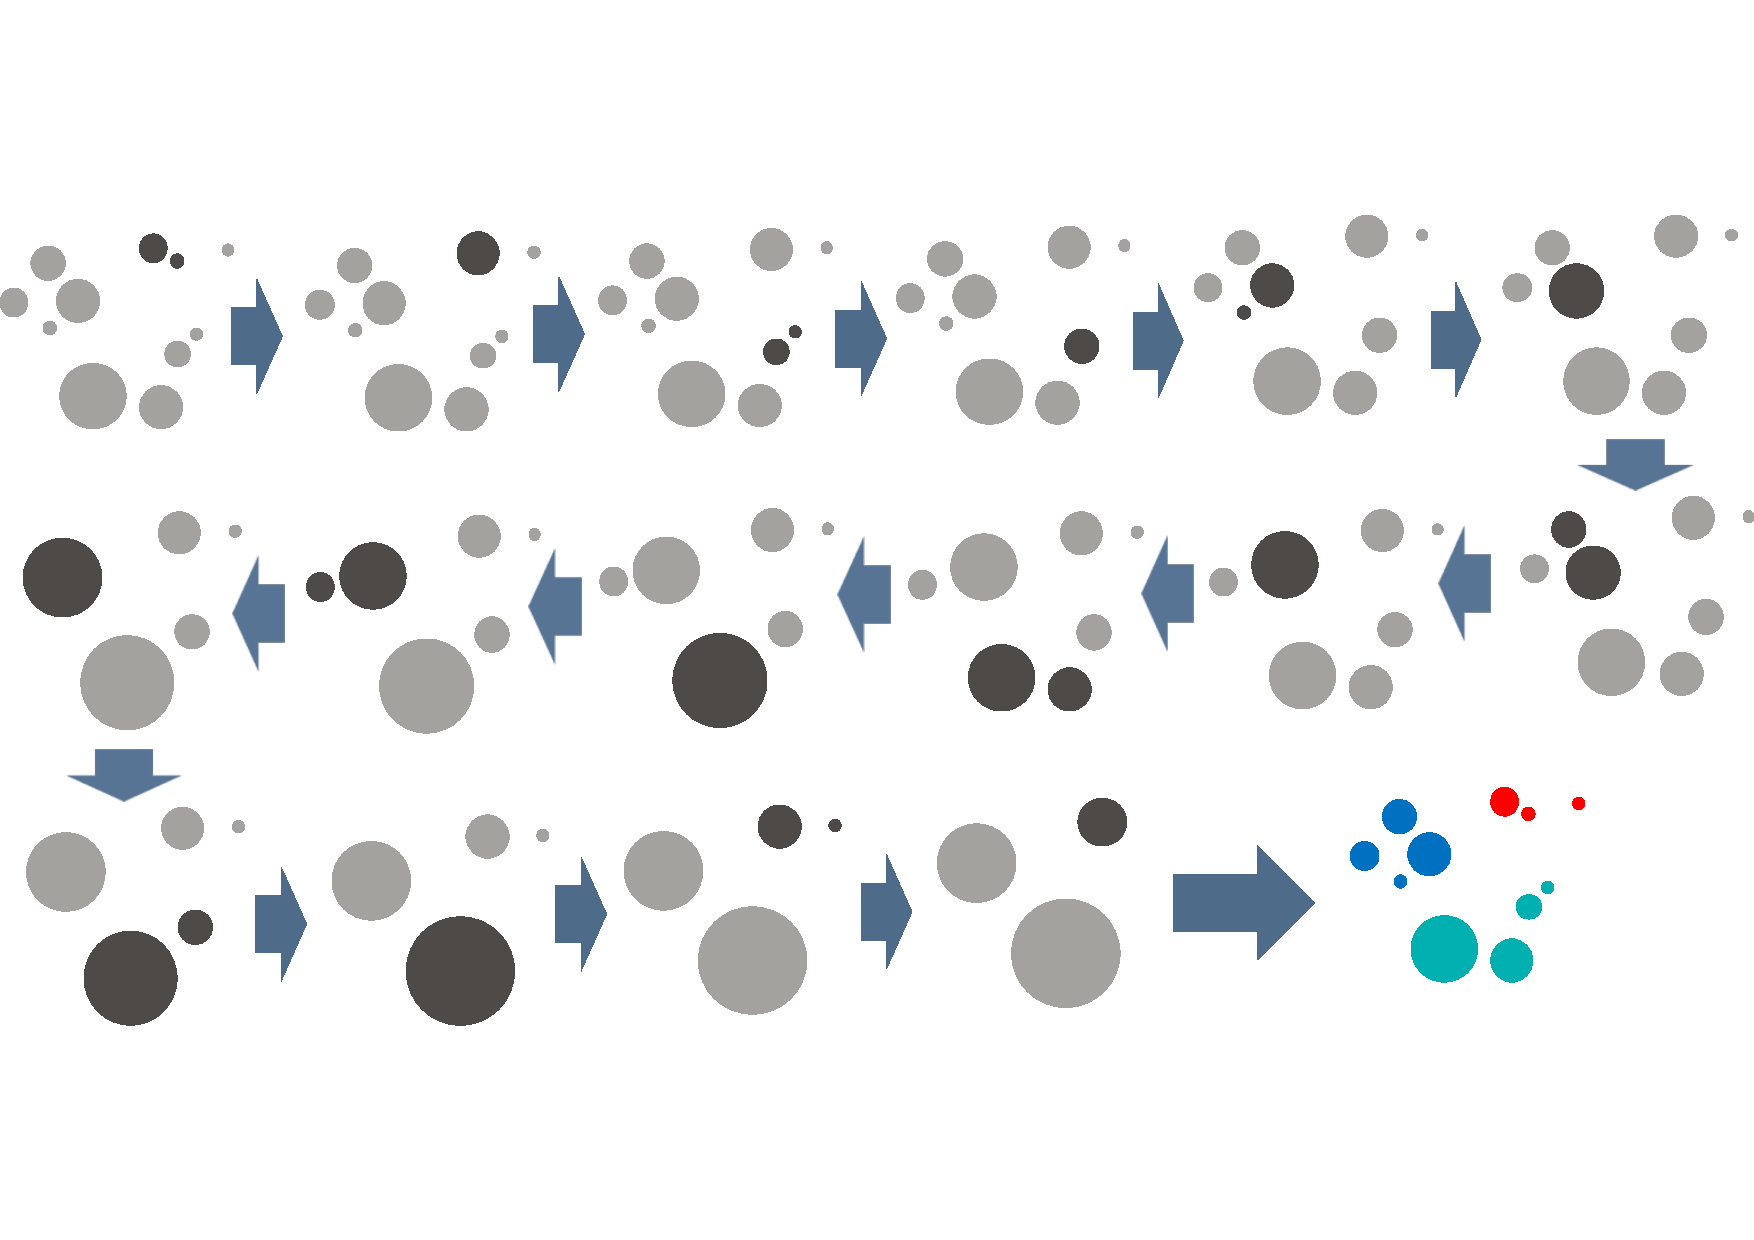
\includegraphics[width=0.85\textwidth]{Figures/PhysObj/jet_algo.pdf}\\
		\caption{Example of constructing protojets to jets}
		\label{PhysObj:fig:jet_algo}
		\end{figure}
		\FloatBarrier

		\begin{figure}[H]
		\centering{}
	    	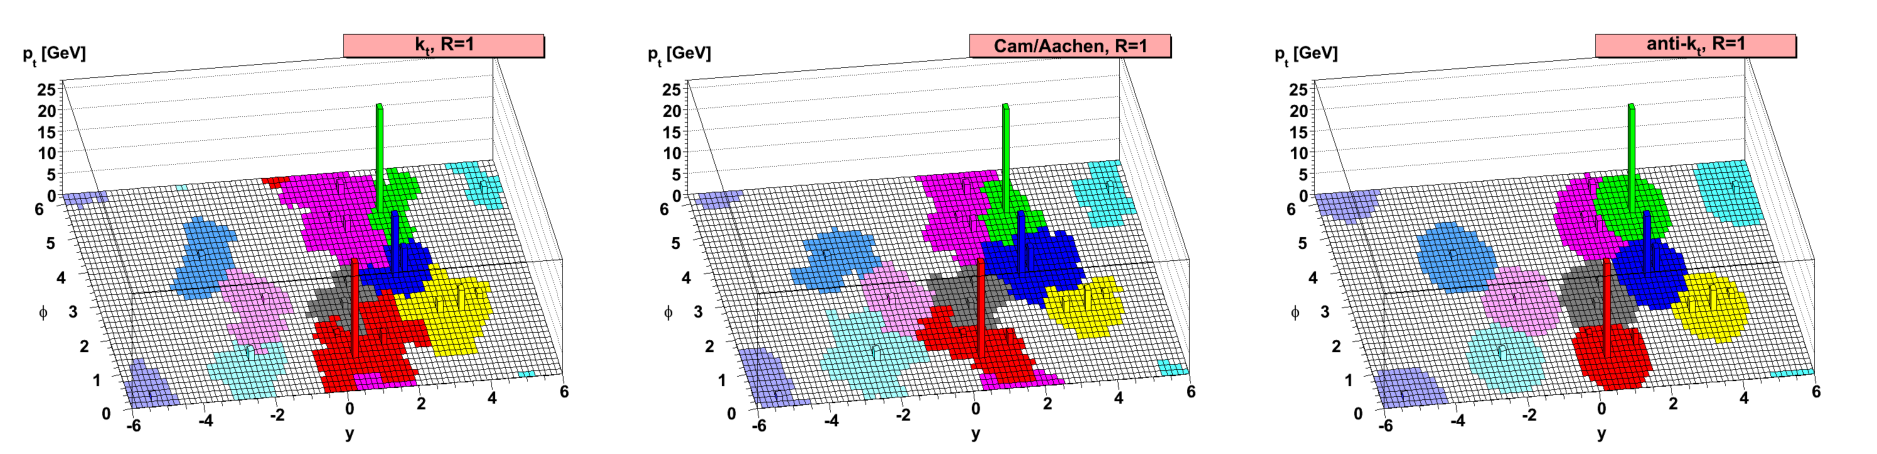
\includegraphics[width=0.85\textwidth]{Figures/PhysObj/3type_jetreco.pdf}\\
		\caption{behavior difference between $k_t$/CA/anti-$k_t$ algorithm \cite{Atkin_2015}}
		\label{PhysObj:fig:3type_jetreco}
		\end{figure}
		\FloatBarrier

		When reconstructing jets, the energy of jets have to be calibrated by jets' $P_T$ and $\eta$. It is named $\textbf{Jet Energy Calibration(Correction)(JEC)}$\cite{collaboration_2011_JEC}. The correction applies a multiplicative factor $C_{cor}$ to the four-monmentum of raw jets. The factor $C_{cor}$ is a product of offset correction, MC calibration factor, absolute energy scale and residuals calibrations. All of the four ingredients are partially relative to jets' $p_T$ and $\eta$.(Eq.\ref{eq:JEC_1})

		\begin{equation}
		\begin{split}
		p_{\mu}^{cor} = C_{cor} \cdot p_{\mu}^{raw} \; \; \; \; \; \; \; \; \; \; \; \; \; \; \; \; \; \; \; \; \; \; \; \; \; \; \; \; \; \; \; \; \; \; \; \; \; \; \; \; \; \; \; \; \; \; \; \; \\
		C_{cor} = C_{offset}(p_T^{raw}) \cdot C_{MC}(p'_T,\eta) \cdot C_{abs}(p''_T) \cdot C_{rel}(\eta)
		\end{split}
		\label{eq:JEC_1}
		\end{equation}
		\FloatBarrier

		In addition to the Jet energy calibrattion, there is also $\textbf{Jet Energy Resolution(JER)}$ considered\cite{JER_twiki}. The issue come from that the jet energy resolution in data is worse than in MC simulation, so we need to correct the resolution in MC with scaling and smearing method to closely describe the data. For a jet, if a well-matched particle-level jet is present(Eq.\ref{eq:JER_0} are the requirements for the matching), the scaling method is adopted. Scaling method scale the four-momentum of jets with a factor $c_{JER}$(Eq.\ref{eq:JER_1}):

		\begin{equation}
		\Delta R < R_{cone}/2, \; \; \; |p_T-p_T^{ptcl}| < 3 \sigma_{JER} \cdot p_T
		\label{eq:JER_0}
		\end{equation}
		\FloatBarrier

		where the $R_{cone}$ is the cone size parameter, in the analysis with AK4 jet, the $R_{cone}$ is 0.4. Also, the $\sigma_{JER}$ is the width which is the resolution measured from MC.

		\begin{equation}
		c_{JER} = 1 + (s_{JER} - 1)\frac{p_T-p_T^{ptcl}}{p_T}
		\label{eq:JER_1}
		\end{equation}
		\FloatBarrier

		The $p_T$ is the transverse momentum of jet, and $p_T^{ptcl}$ is the transverse momentum of the corresponding jet clustered from generator-level particles. $s_{JER}$ is the data-to-MC core resolution scale factor. If the $c_{JER}$ is measured negative, it is set to be zero, that is to say, the factor $c_{JER}$ truncated at zero; In the other case that doesn't require the presence of well-match jet, it is set to adopt the smearing method(Eq.\ref{eq:JER_2}):

		\begin{equation}
		c_{JER} = 1 + N(0,\sigma_{JER})\sqrt{max(s_{JER}^2-1,0)}
		\label{eq:JER_2}
		\end{equation}
		\FloatBarrier

		The selected jets in the analysis comply with the criteria below:

		\begin{itemize}
		\item $p_T$ > 30GeV
		\item $|\eta|$ < 2.4
		\item $\Delta R$ < 0.4 with the selected lepton
		\item pass Jet Loose ID : \cite{JetLooseID_twiki}
		\begin{itemize}
			\item neutral hadron energy fraction < 0.99
			\item neutral EM fraction < 0.99
			\item charged hadron fraction > 0
			\item number of constituents > 1
			\item charge multiplicity > 0
			\item charged EM fraction < 0.99
		\end{itemize}
		\label{PhysObj:itm:sel_jet}
		\end{itemize}
		

		\subsubsection{b-tagged jet}
		\label{sssec:bjet}

			To precisely identify the type of original particle of jets, some algorithm are computed to be a discriminator. Instead of light-flavor(udsg), there are commonly heavy-flavor(b,c) jet discriminator using some variables to identify the properties of jets from the radiation and hadronization of b or c quarks, for example, the hadrons containing b quark's lifetime is more longer than ones with c quarks. In this analysis, b-quark discriminator is handed to pick up the b quarks decaying from t quarks. According to the long lifetime of b hadrons, this would cause displacements of a few mm to one cm for b hadrons. The displaced tracks construct the secondary vertex(SV). The illustration diagram of primary vertex and secondary vertex is shown in Fig.\ref{PhysObj:fig:PV_SV}. 

			\begin{figure}[H]
			\centering{}
		    	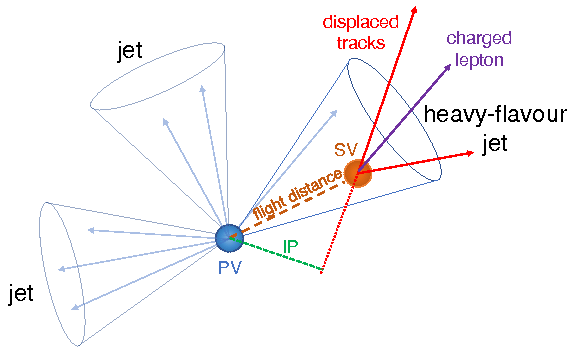
\includegraphics[width=0.85\textwidth]{Figures/PhysObj/PV_SV.png}\\
			\caption{Illustration of useful variables for b tagging \cite{CMS-BTV-16-002}}
			\label{PhysObj:fig:PV_SV}
			\end{figure}
			\FloatBarrier

			The displacemennt of tracks themselves would be characterized by their impact parameters. Moreover, all the relative information are used to compute to be a dicriminator factor with multi-variated classifying method, forr example, the secondary vertex mass is also used. The technique is called $\textbf{combine secondary vertex(CSV) discriminator}$. There are more type of CSV discriminator, the chosen one in this analysis is $\textbf{DeepCSV}$ modified by CSVv2 algorithm. The inclusive vertex finding (IVF) algorithm was the standard SV reconnstruction algorithm, and DeepCSV apply the same tracks and IVF as the CSVv2 tagger. The difference of DeepCSV is that the trrack-based variables up to six tracks are used in training. Moreover, the improvemence of deepCSV is using a deep neural network with more hidden layers and a simultaneous training in all vertex categories and all jets' flavors to train the classification algorithm. The previous information and more details about CSV, CSVv2, and DeepCSV can be approached in the reference \cite{CMS-PAS-BTV-15-001} and \cite{CMS-BTV-16-002}.

			The training of the deep neural network is done under four hidden layers with 100 nodes which are fully connected. The output layers includes five nodes, that is, five jet flavor categories. Those five categories are defined whether the jets contains -- exactly one b hadron, at least two b hadrons, no b hadrons and exactly one c hadron, no b hadrons and at least two c hadrons, and others. At the last layer's nodes, there are the intepretation of output values with probability for certain jet flavor category -- P($\emph{f}$), which could be looked as the discriminators and so could combined one. The following are the distributions of each categories' discriminators and the jets-categorized performance(Fig.\ref{PhysObj:fig:flavor_discr}):

			\begin{figure}[H]
			\centering
			    \subfigure{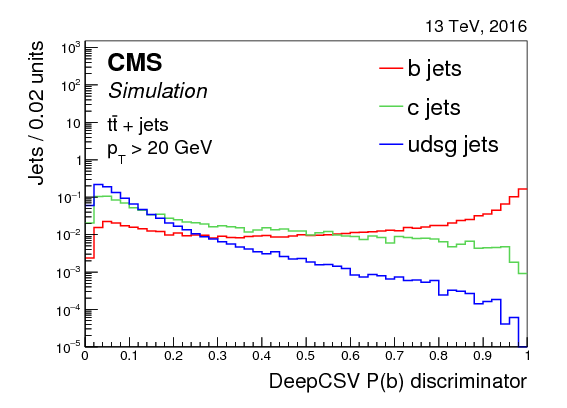
\includegraphics[width=0.45\textwidth]{Figures/PhysObj/deepCSV_b.png}}
			    \subfigure{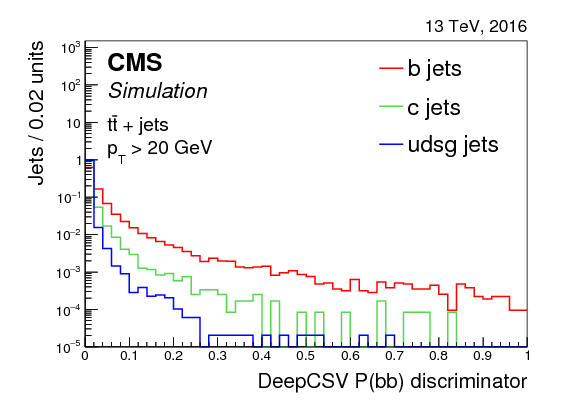
\includegraphics[width=0.45\textwidth]{Figures/PhysObj/deepCSV_bb.png}}\\
			\end{figure}
			\FloatBarrier
			\begin{figure}[H]
			\centering
			    \subfigure{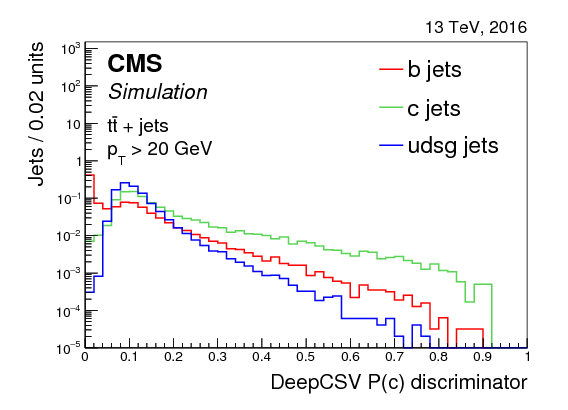
\includegraphics[width=0.45\textwidth]{Figures/PhysObj/deepCSV_c.png}}
			    \subfigure{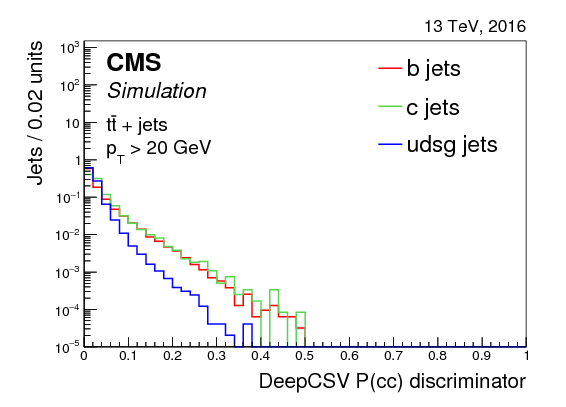
\includegraphics[width=0.45\textwidth]{Figures/PhysObj/deepCSV_cc.png}}\\
			\end{figure}
			\FloatBarrier
			\begin{figure}[H]
			\centering
			    \subfigure{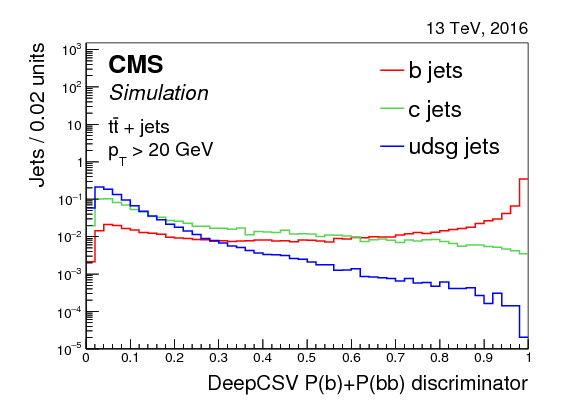
\includegraphics[width=0.65\textwidth]{Figures/PhysObj/deepCSV_b_bb.png}}\\
			\caption{Distribution of the DeepCSV P($b$), P($bb$), P($c$), P($cc$), P($b$) + P($bb$) discriminator values for jets of different flavors in $t\bar{t}$ events. Reference by \cite{CMS-BTV-16-002}}
			\label{PhysObj:fig:flavor_discr}
			\end{figure}
			\FloatBarrier

			The P($b$) + P($bb$) discriminator is used in the usual physics analysis with DeepCSV values. The DeepCSV b-tagging algorithm is used on the jets which passed the jet selection. In this analysis, there are two criteria would be used -- DeepCSV Medium(which is used in signal region) and DeepCSV Loose(which is used in control region). The criteria is applying thresholds on DeepCSV value, the thresholds are shown below:

			\begin{itemize}
				\item DeepCSV Medium $\rightarrow$ Discriminator of DeepCSV is above 0.6321
				\item DeepCSV Loose $\rightarrow$ Discriminator of DeepCSV is within 0.2217-0.6321
			\label{PhysObj:itm:btag}
			\end{itemize}

	\subsection{Trigger}
	\label{ssec:PhysObj_trg}





\FloatBarrier
